\chapter{Estado del Arte}
\thispagestyle{empty}

En el campo del aprendizaje automático, el tema de la estimación de la distancia en fotografías faciales ha ganado recientemente mucha atención. Se puede observar en la Figura \ref{fig5} la cantidad de publicaciones existentes en la base de datos Scopus \footnote{Las búsquedas se pueden consultar en el apéndice} que hacen referencia a la estimación del SCD. Hay 430 publicaciones registradas desde 1992.

El número de publicaciones relacionadas con este tema, va aumentando a lo largo del tiempo, llegando a obtener un mayor número de publicaciones en 2020. Pese al aumento de publicaciones en este ámbito, es a partir del 2015 cuando se empiezan a aplicar las técnicas de deep learning. Este aumento está relacionado con los avances tecnológicos que permiten aplicar nuevas técnicas y conocimientos. 

\begin{figure}[h]
	\centering
	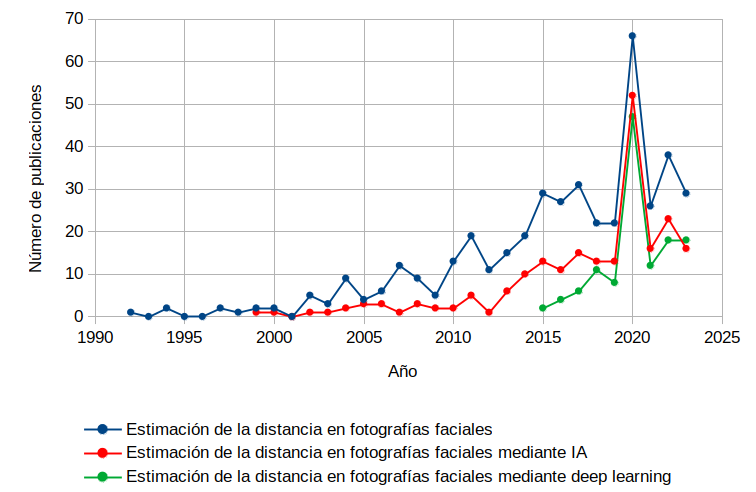
\includegraphics[scale=0.45]{imagenes/cap3/grafica_scopus3.png}
	\caption{Número de publicaciones, en Scopus, relacionadas con la estimación de la distancia en fotografías faciales en función del año de publicación}
	\label{fig5}
\end{figure}

\section{Primeros enfoques}

El primer método utilizado para abordar la estimación métrica del SCD fue propuesto por \cite{28}, se basa en el uso de un conjunto de puntos de referencia de la cara para estimar la pose y la distancia a la cámara en distancias desde 10 cm hasta 3 m. El proceso consiste en, entrenar un modelo de regresión para predecir la distancia entre la cámara y la cara, utilizando un conjunto de imágenes 3D de caras humanas con sus respectivos puntos de referencia faciales (se observa que estas referencias no varían drásticamente entre individuos, sino que se agrupan en 'clusters'). Dicho conjunto de datos 3D solo contiene vistas de frontales y de perfil 3/4. 

Dada una imagen 2D de una cara desconocida, se identifican los puntos de referencia faciales y mediante el algoritmo EPnP \cite{29}, junto con la suposición de que las referencias no varían mucho entre individuos, se infiere la pose 3D de la cara y se utiliza el modelo de regresión previamente entrenado para predecir el valor de la distancia a la cámara.

Algunas de las limitaciones asociados a este primer método son: el uso de un conjunto de datos 3D (no siempre tendremos disponibles imágenes 3D para el entrenamiento), la combinación de diferentes longitudes focales en el mismo dataset o el reconocimiento manual de los puntos de referencia faciales

Posteriormente, \cite{30} propuso un método que no necesitaba la reconstrucción 3D ni la anotación manual de los puntos de referencia de la imagen. Este método utiliza un conjunto de datos llamado Caltech Multi-Distance Portraits (CMDP), compuesto de 53 retratos individuales desde 7 distancias distintas entre 60 cm y 480 cm, para entrenar el modelo. Todas las imágenes del conjunto de datos fueron anotadas manualmente con 55 marcas faciales. 

El método se basa en dos fases: primero, la identificación automática de los puntos de referencia faciales, y después, la estimación de la distancia mediante regresión.

Este nuevo enfoque, a pesar de mejorar lo que previamente se había hecho, sigue teniendo algunas limitaciones como el recorte de las imágenes (pérdida de resolución) o la única vista frontal.

Existen otros métodos que estiman el SCD a partir de características anatómicas como el tamaño de la cara, la distancia de los ojos o una combinación de ambos. NO TENGO ACCESO A LOS PDFS

\section{Mediapipe}


\section{PerspectiveX}

PerspectiveX fue el método propuesto por Stephan en \cite{31} para la estimación del SCD en fotografías faciales con el fin de mejorar el proceso de superposición craneofacial.

\section{FacialSCDnet}


